\begin{figure}[h]
    \centering
    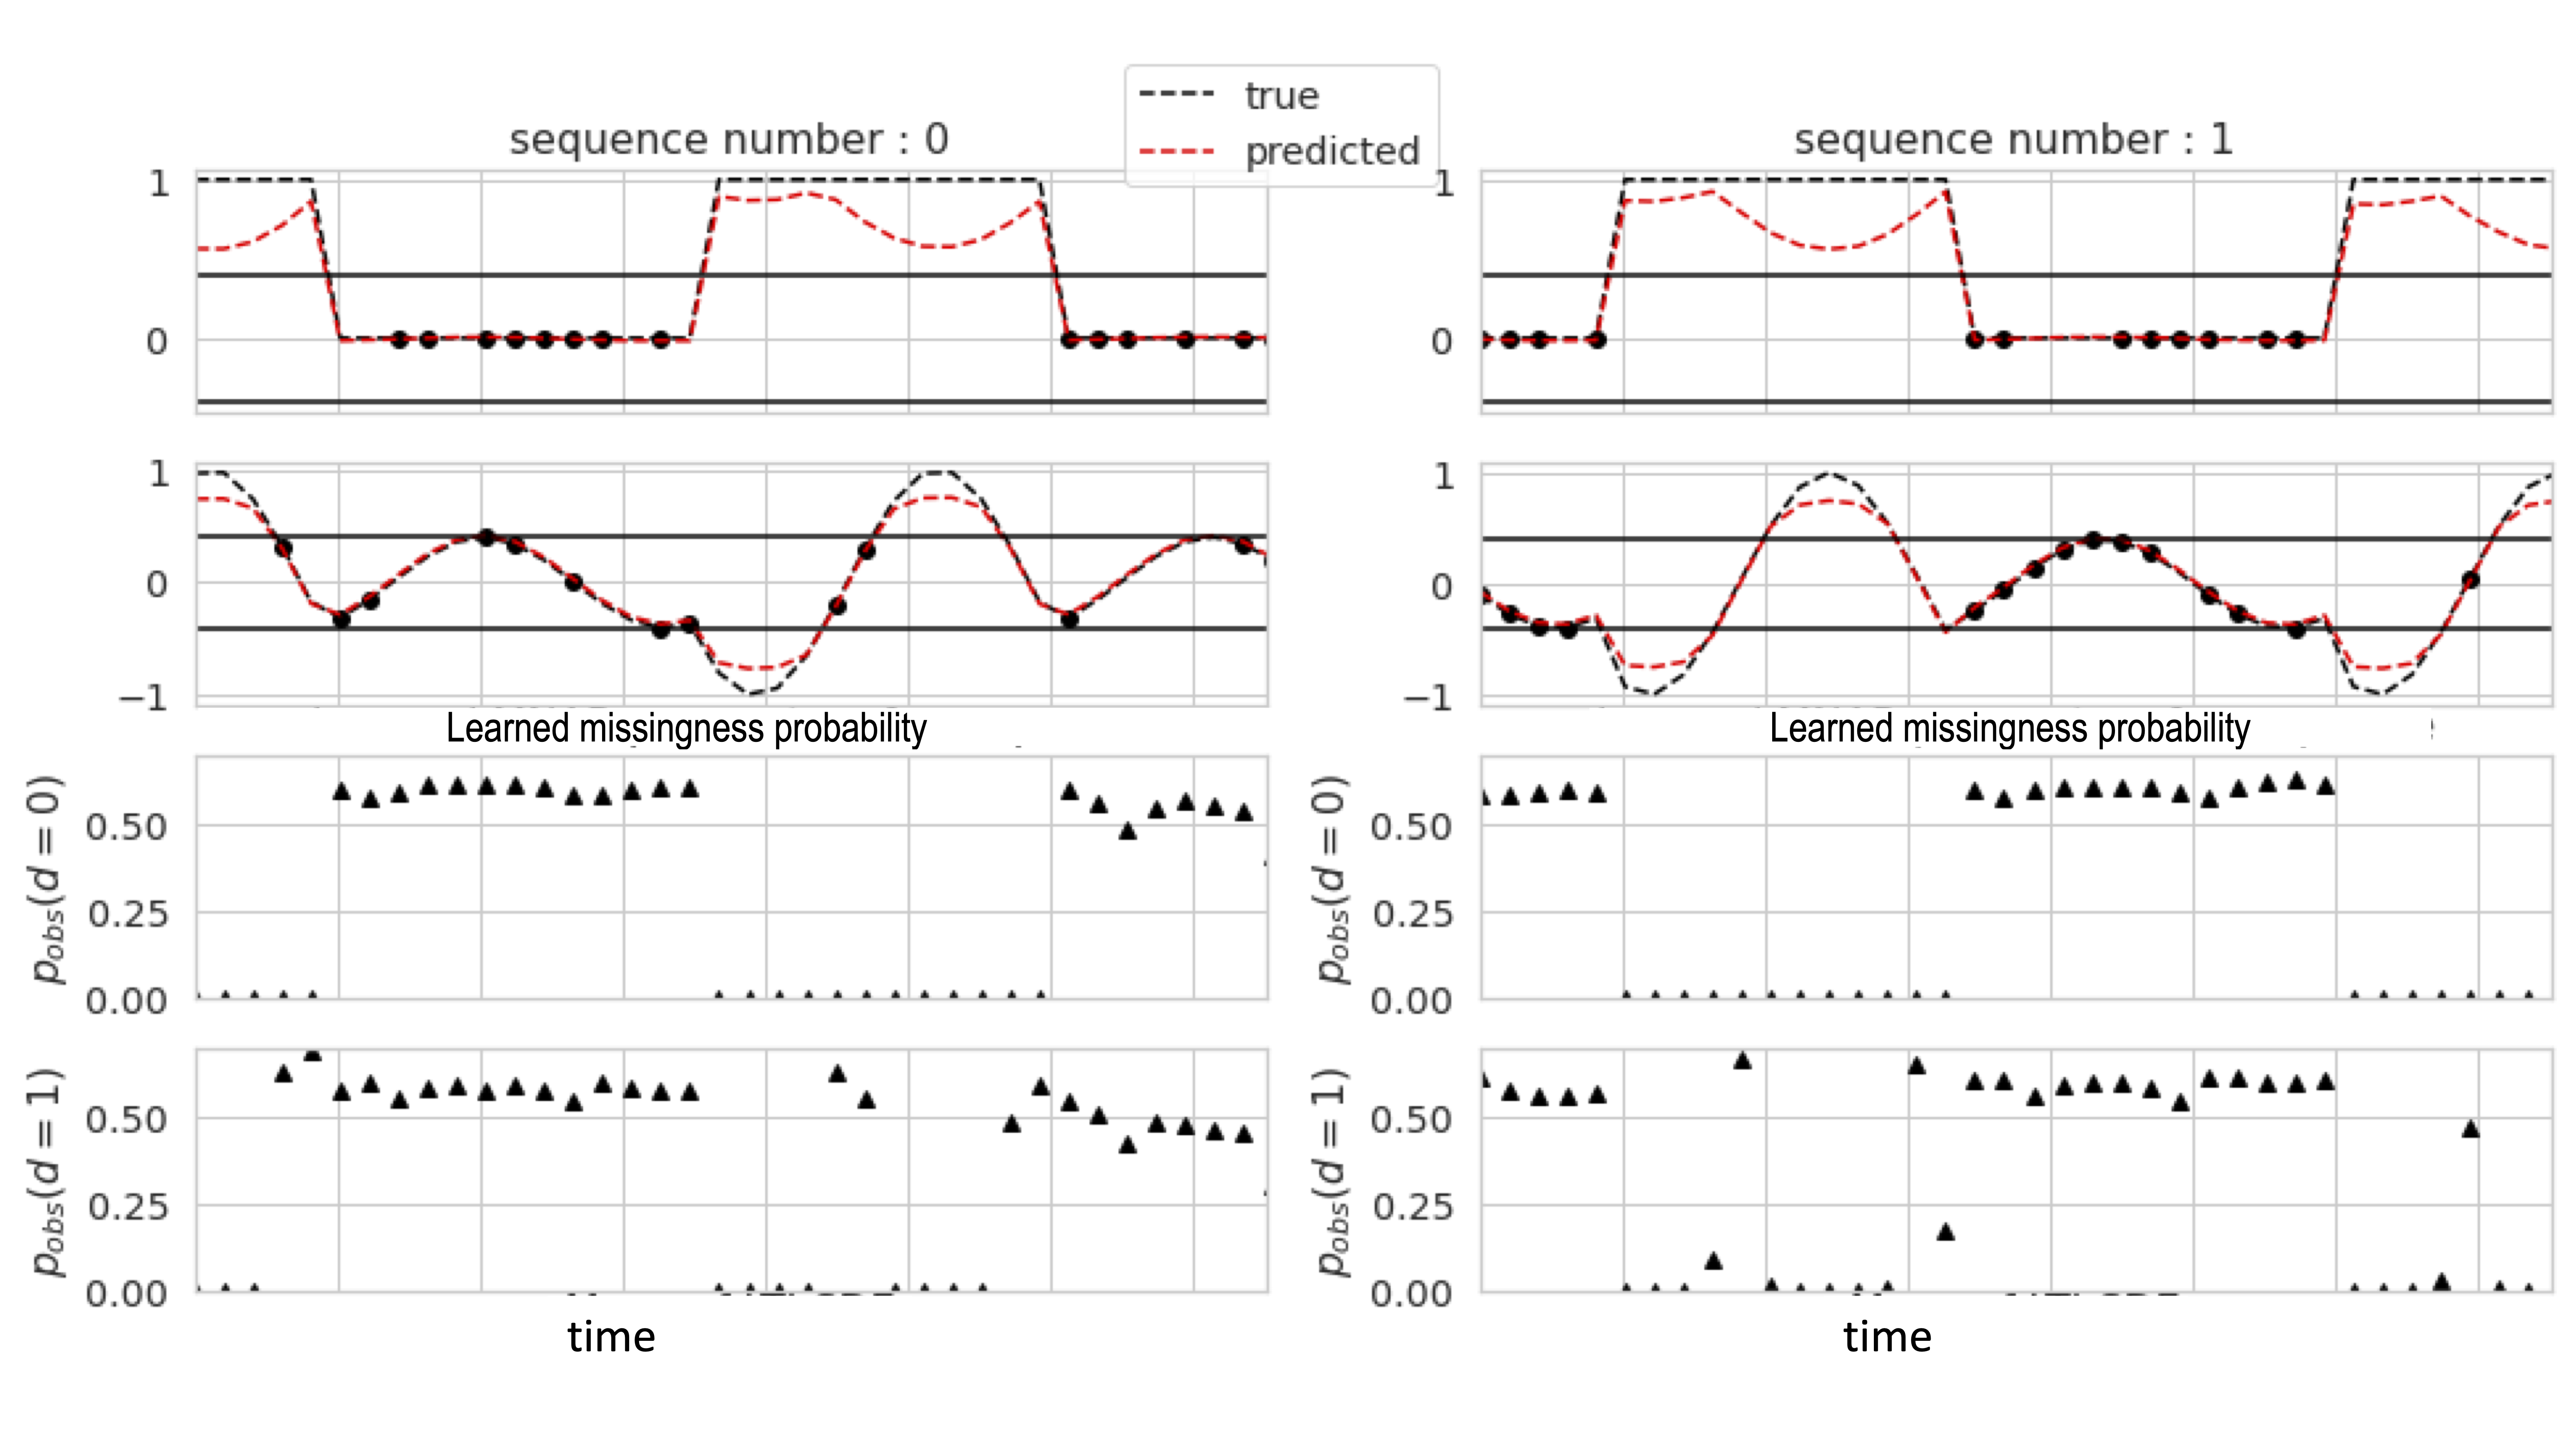
\includegraphics[width=1.0\textwidth]{content/chapters/irregular_time_series_data_driven_missingness/figures/learning_mnar_mechanism.png}
    \caption[Demonstration of our CRU-FM model’s ability to learn the data-dependent missingness mechanism]{Demonstration of our CRU-FM model's ability to learn the data-dependent missingness mechanism. \textit{Top 2 rows : } We show the 2 channels of data from 2 representative sequences from our toy experiment (details in section \ref{sec:synthetic_experiment}). The black dashed line and the red dashed line represent the true and reconstructed sequences respectively. The black dots represent the observed values at irregularly spaced timepoints. \textit{Bottom 2 rows : } Learned probabilities of observing a measurement in each of the channels above.
    Remember, we set the data-dependent missingness mechanism as follows : the probability of observing a value outside the dashed black lines for each channel is 0.0006 and the probability of observing a measurement within the dashed black lines is 0.6. This mechanism is learned by our model (the black upward arrows show the learned probabilities of observing a value). The ability of our model to learn these data-dependent missingness mechanisms leads to improved downstream extrapolation performance.}
    \label{fig:learning_missingness_mechanism}
\end{figure}